\documentclass[../../main.tex]{subfiles}
\begin{document}

{\bf [解]}
題意より
\begin{align}
 a,b >0 \label{eq:1}
\end{align}
の元で考える．

\paragraph{(1)}

与えられた関数$f(x)=\dfrac{x^4}{(x-a)^3}$は$x>a$で正であるから両辺自然対数をとると
\begin{align}
 \log f(x)=4\log x-3\log(x-a) 
\end{align}
だから，この両辺を$x$で微分して
\begin{align}
\begin{split}
\dfrac{f'(x)}{f(x)}&=\dfrac{4}{x}-\dfrac{3}{x-a}=\dfrac{x-4a}{x(x-a)} \\
\therefore\ f'(x) &=\dfrac{x^3(x-4a)}{(x-a)^4}
\end{split}
\end{align}
となる．$x>a$では$x^3>0,\ (x-a)^4>0$だから，$f'(x)$の符号は$(x-4a)$の符号と一致する．
従って$f(x)$の増減表は以下の通りである．

\begin{table}[htb]
  \centering
\caption{$f(x)$の増減表}
\begin{tabular}{c|ccccc}
$x$ & $a$ & & $4a$ & & \\
\hline
$f'$ & & $-$ & $0$ & $+$ & \\
\hline
$f$ & & $\searrow$ & & $\nearrow$ &
\end{tabular}
\end{table}

すなわち，$f$は$a<x<4a$で単調減少，$4a<x$で単調増加し，$x=4a$で最小値$f(4a)=\dfrac{(4a)^4}{(3a)^3}=\dfrac{4^4}{3^3}a$をとる．

\begin{figure}[htb]
\begin{center}
\begin{tikzpicture}[xscale=1.4, yscale=0.5, >=stealth]

  % --- 1. 座標軸 ---
  \draw[->, thick] (-0.3, 0) -- (5.5, 0) node[right] {$x$};
  \draw[->, thick] (0, -0.4) -- (0, 15) node[above] {$y$};
  \node[below left, font=\small] at (0,0) {$O$};

  % パラメータ (a = 0.8 のスケール例)
  \def\aVal{0.8}
  \pgfmathsetmacro{\minX}{4*\aVal}          % 4a = 3.2
  \pgfmathsetmacro{\minY}{(256/27)*\aVal} % 描画用にスケーリングした極小値

  % --- 2. 漸近線 x = a ---
  \draw[dashed, red!80!black, thick] (\aVal, -0.3) -- (\aVal, 15)
    node[above, font=\small] {$x = a$};
  \node[below, font=\small] at (\aVal, 0) {$a$};

  % --- 3. グラフ y = f(x) (x > a) ---
  \draw[ultra thick, blue!80!black, domain=1.5:5.0, samples=80] 
    plot (\x, { (\x^4 / ((\x - \aVal)^3)) }) 
    node[right, font=\small] {$y = f(x)$};

  % --- 4. 極小値 (4a, f(4a)) のプロットとガイド線 ---
  \coordinate (MinPt) at ({\minX}, {\minY});
  \draw[dashed, gray] ({\minX}, 0) node[below, black, font=\small] {$4a$} -- (MinPt);
  \draw[dashed, gray] (0, {\minY}) node[left, black, font=\small] {$\dfrac{4^4}{27}a$} -- (MinPt);
  
  \fill[red!80!black] (MinPt) circle (2pt);
  % \node[red!80!black, font=\scriptsize, above right] at (MinPt) {極小（最小）};

\end{tikzpicture}
\end{center}
\caption{$f(x)$（$x > a$）の概形}
\end{figure}

\paragraph{(2)}

与えられた関数
\begin{align}
 g(x)=\dfrac{1}{(x-a)^2}-\dfrac{b}{x^3} \label{eq:2}
\end{align}
の一階微分は
\begin{align}
 g'(x)=\dfrac{-2}{(x-a)^3}+\dfrac{3b}{x^4} \label{eq:3}
\end{align}
である．

$y=g(x)$が$x$軸に平行な直線と3点で交わるためには，$a<x$なる$x$で$g'(x)=0$でかつこの前後で$g'$が符号を変えるようなものが少なくとも$2$つあることが必要である．そこで$g'(x)$の符号を考えるため\cref{eq:3}を変形すると
\begin{align}
 g'(x)
  &= \dfrac{2}{x^4}\left(\dfrac{3b}{2} - \dfrac{x^4}{(x-a)^3} \right) \\
  &=  \dfrac{2}{x^4}\left(\dfrac{3b}{2} - f(x) \right) \label{eq:4}
\end{align}
となり，$0<a<x$におけるこの符号は
\begin{align}
 h(x) = \dfrac{3b}{2} - f(x)
\end{align}
と等しい．(1)の結果より$f(x)$は極小値を一つだけ持ち，その値は
\begin{align}
 f\left(4a\right) = \dfrac{4^4 a}{3^3} 
\end{align}
だから$h(x)=0$かつ前後で$h'(x)$が符号を変える$x$が少なくとも二つある条件はこれより$\dfrac{3b}{2}$が大きいことで
\begin{align}
 \dfrac{3b}{2} > \dfrac{4^4 a}{3^3} \iff  b > \dfrac{2\cdot 4^4}{3^4}a \label{eq:5}
\end{align}
である．

\begin{figure}[htb]
\begin{center}
\begin{tikzpicture}[xscale=1.4, yscale=0.5, >=stealth]

  % --- 1. 座標軸 ---
  \draw[->, thick] (-0.3, 0) -- (5.5, 0) node[right] {$x$};
  \draw[->, thick] (0, -0.4) -- (0, 15) node[above] {$y$};
  \node[below left, font=\small] at (0,0) {$O$};

  % パラメータ (a = 0.8 のスケール例)
  \def\aVal{0.8}
  \pgfmathsetmacro{\minX}{4*\aVal}          % 4a = 3.2
  \pgfmathsetmacro{\minY}{(256/27)*\aVal} % 描画用にスケーリングした極小値


  % 漸近線 x = a
  \draw[dashed, gray] (\aVal, -0.3) -- (\aVal, 15) node[above, font=\scriptsize] {$x = a$};
  \node[below, font=\small] at (\aVal, 0) {$a$};

  % グラフ y = f(x)
  \draw[ultra thick, blue!80!black, domain=1.5:5.0, samples=80] 
    plot (\x, { (\x^4 / ((\x - \aVal)^3)) })
    node[right, font=\small] {$y = f(x)$};

  % 直線 y = 3b/2 (極小値より上)
  \def\yLine{8}
  \draw[thick, red!80!black] (0.5, \yLine) -- (5.2, \yLine)
    node[below right, font=\small] {$y = \dfrac{3b}{2}$};

  % 極小値レベル (破線)
  \coordinate (MinPt) at ({\minX}, {\minY});
  \draw[dashed, gray!70] (0, {\minY}) node[left, font=\scriptsize] {$f(4a)$} -- (MinPt);
  \draw[dashed, gray!70] ({\minX}, 0) node[below, font=\scriptsize] {$4a$} -- (MinPt);

  % 交点 alpha, beta
  \coordinate (Palpha) at (2.4, \yLine);
  \coordinate (Pbeta)  at (4.4, \yLine);

  \draw[dashed, purple!80!black] (2.4, 0) node[below, font=\small, text=purple!80!black] {$\alpha$} -- (Palpha);
  \draw[dashed, purple!80!black] (4.4, 0) node[below, font=\small, text=purple!80!black] {$\beta$} -- (Pbeta);

  \fill[purple!80!black] (Palpha) circle (1.8pt);
  \fill[purple!80!black] (Pbeta)  circle (1.8pt);

  % g'(x) の符号領域表示
  \node[red!80!black, font=\scriptsize] at (1.1, 2.7) {$g'<0$};
  \node[blue!80!black, font=\scriptsize] at (3.2, 2.5) {$g'>0$ ($\frac{3b}{2} > f$)};
  \node[red!80!black, font=\scriptsize] at (4.9, 2.7) {$g'<0$};

\end{tikzpicture}
\end{center}
\caption{$y = f(x)$ と直線 $y = \dfrac{3b}{2}$ の交点 $\alpha, \beta$（$g'(x)=0$ の解）}
\end{figure}

この時グラフより$h'(x)=0$，従って$g'(x)=0$は2解$\alpha,\beta$（$\alpha<\beta$）を持ち，$g(x)$の増減表は以下のようになる．

\begin{table}[htb]
  \centering
\caption{$g(x)$の増減表}
\begin{tabular}{c|ccccccc}
$x$ & $a$ & & $\alpha$ & & $\beta$ & & \\
\hline
$g'$ & & $-$ & $0$ & $+$ & $0$ & $-$ & \\
\hline
$g$ & & $\searrow$ & & $\nearrow$ & & $\searrow$ &
\end{tabular}
\end{table}

$g(x)\to+\infty\ (x\to a^+)$，$g(x)\to0\ (x\to+\infty)$だから，$g$のグラフは，$+\infty$から$g(\alpha)$（極小）まで減少，$g(\beta)$（極大）まで増加，その後$0$に向かって減少する形になる．この時，$\max\left(g(\alpha),0\right)<k<g(\beta)$をみたす$k$に対し，直線$y=k$は$g$のグラフとちょうど3点で交わるから条件は十分である．

\begin{figure}[htb]
\begin{center}
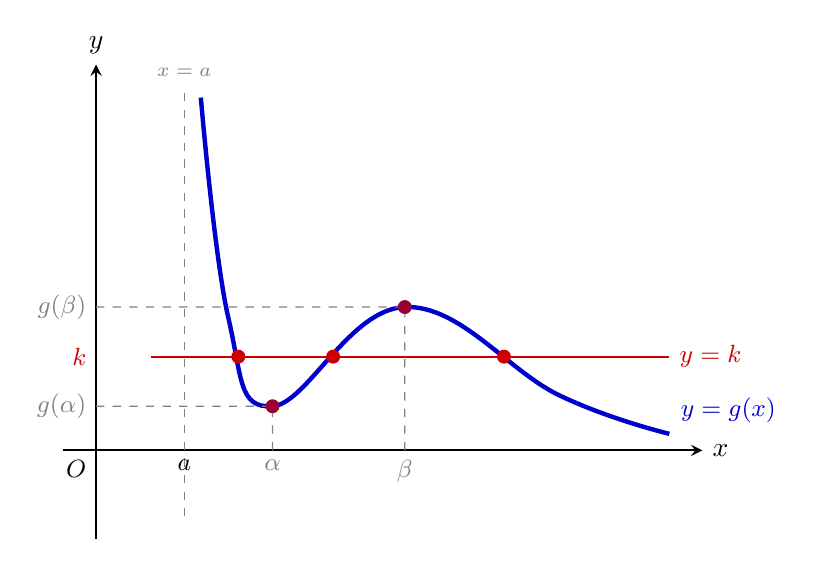
\begin{tikzpicture}[scale=1.4, >=stealth]

  % --- 1. 座標軸 ---
  \draw[->, thick] (-0.3, 0) -- (5.5, 0) node[right] {$x$};
  \draw[->, thick] (0, -0.8) -- (0, 3.5) node[above] {$y$};
  \node[below left, font=\small] at (0,0) {$O$};

  \def\aVal{0.8}

  % 漸近線 x = a
  \draw[dashed, gray] (\aVal, -0.6) -- (\aVal, 3.3) node[above, font=\scriptsize] {$x = a$};
  \node[below, font=\small] at (\aVal, 0) {$a$};

  % --- 2. 曲線 y = g(x) の描画 (滑らかな曲線でプロット) ---
  \draw[ultra thick, blue!80!black] 
    plot[smooth, tension=0.7] coordinates {
      (0.95, 3.2) (1.2, 1.2) (1.6, 0.4) (2.8, 1.3) (4.2, 0.5) (5.2, 0.15)
    } node[above right, font=\small] {$y = g(x)$};

  % 極小点 (alpha, g(alpha))
  \coordinate (Galpha) at (1.6, 0.4);
  \draw[dashed, gray] (1.6, 0) node[below, font=\small] {$\alpha$} -- (Galpha);
  \draw[dashed, gray] (0, 0.4) node[left, font=\small] {$g(\alpha)$} -- (Galpha);
  \fill[purple!80!black] (Galpha) circle (1.8pt);

  % 極大点 (beta, g(beta))
  \coordinate (Gbeta) at (2.8, 1.3);
  \draw[dashed, gray] (2.8, 0) node[below, font=\small] {$\beta$} -- (Gbeta);
  \draw[dashed, gray] (0, 1.3) node[left, font=\small] {$g(\beta)$} -- (Gbeta);
  \fill[purple!80!black] (Gbeta) circle (1.8pt);

  % --- 3. 3交点をもつ直線 y = k ( g(alpha) < k < g(beta) ) ---
  \def\kVal{0.85}
  \draw[thick, red!80!black] (0.5, \kVal) -- (5.2, \kVal) 
    node[right, font=\small] {$y = k$};
  \node[left, red!80!black, font=\small] at (0, \kVal) {$k$};

  % 3つの交点のプロット
  \fill[red!80!black] (1.29, \kVal) circle (1.8pt);
  \fill[red!80!black] (2.15, \kVal) circle (1.8pt);
  \fill[red!80!black] (3.70, \kVal) circle (1.8pt);

\end{tikzpicture}
\end{center}
\caption{$y = g(x)$ の概形と 3 点で交わる直線 $y = k$}
\end{figure}

以上から，もとめる必要十分条件は\cref{eq:5}で，
\begin{align}
b>\dfrac{2\cdot4^4}{3^4}a
\end{align}
となる．

\newpage

\end{document}
